\documentclass[class=../../report, crop=false]{standalone}
\usepackage{graphicx}
\usepackage{mathtools}
\usepackage{float}
\usepackage{rotating}
\usepackage{caption}

\begin{document}
\section{Pugh Charts} \label{app:pugh}
\mbox{} \begin{center}
	\begin{sideways}
		\begin{minipage}{1.1\textwidth}
			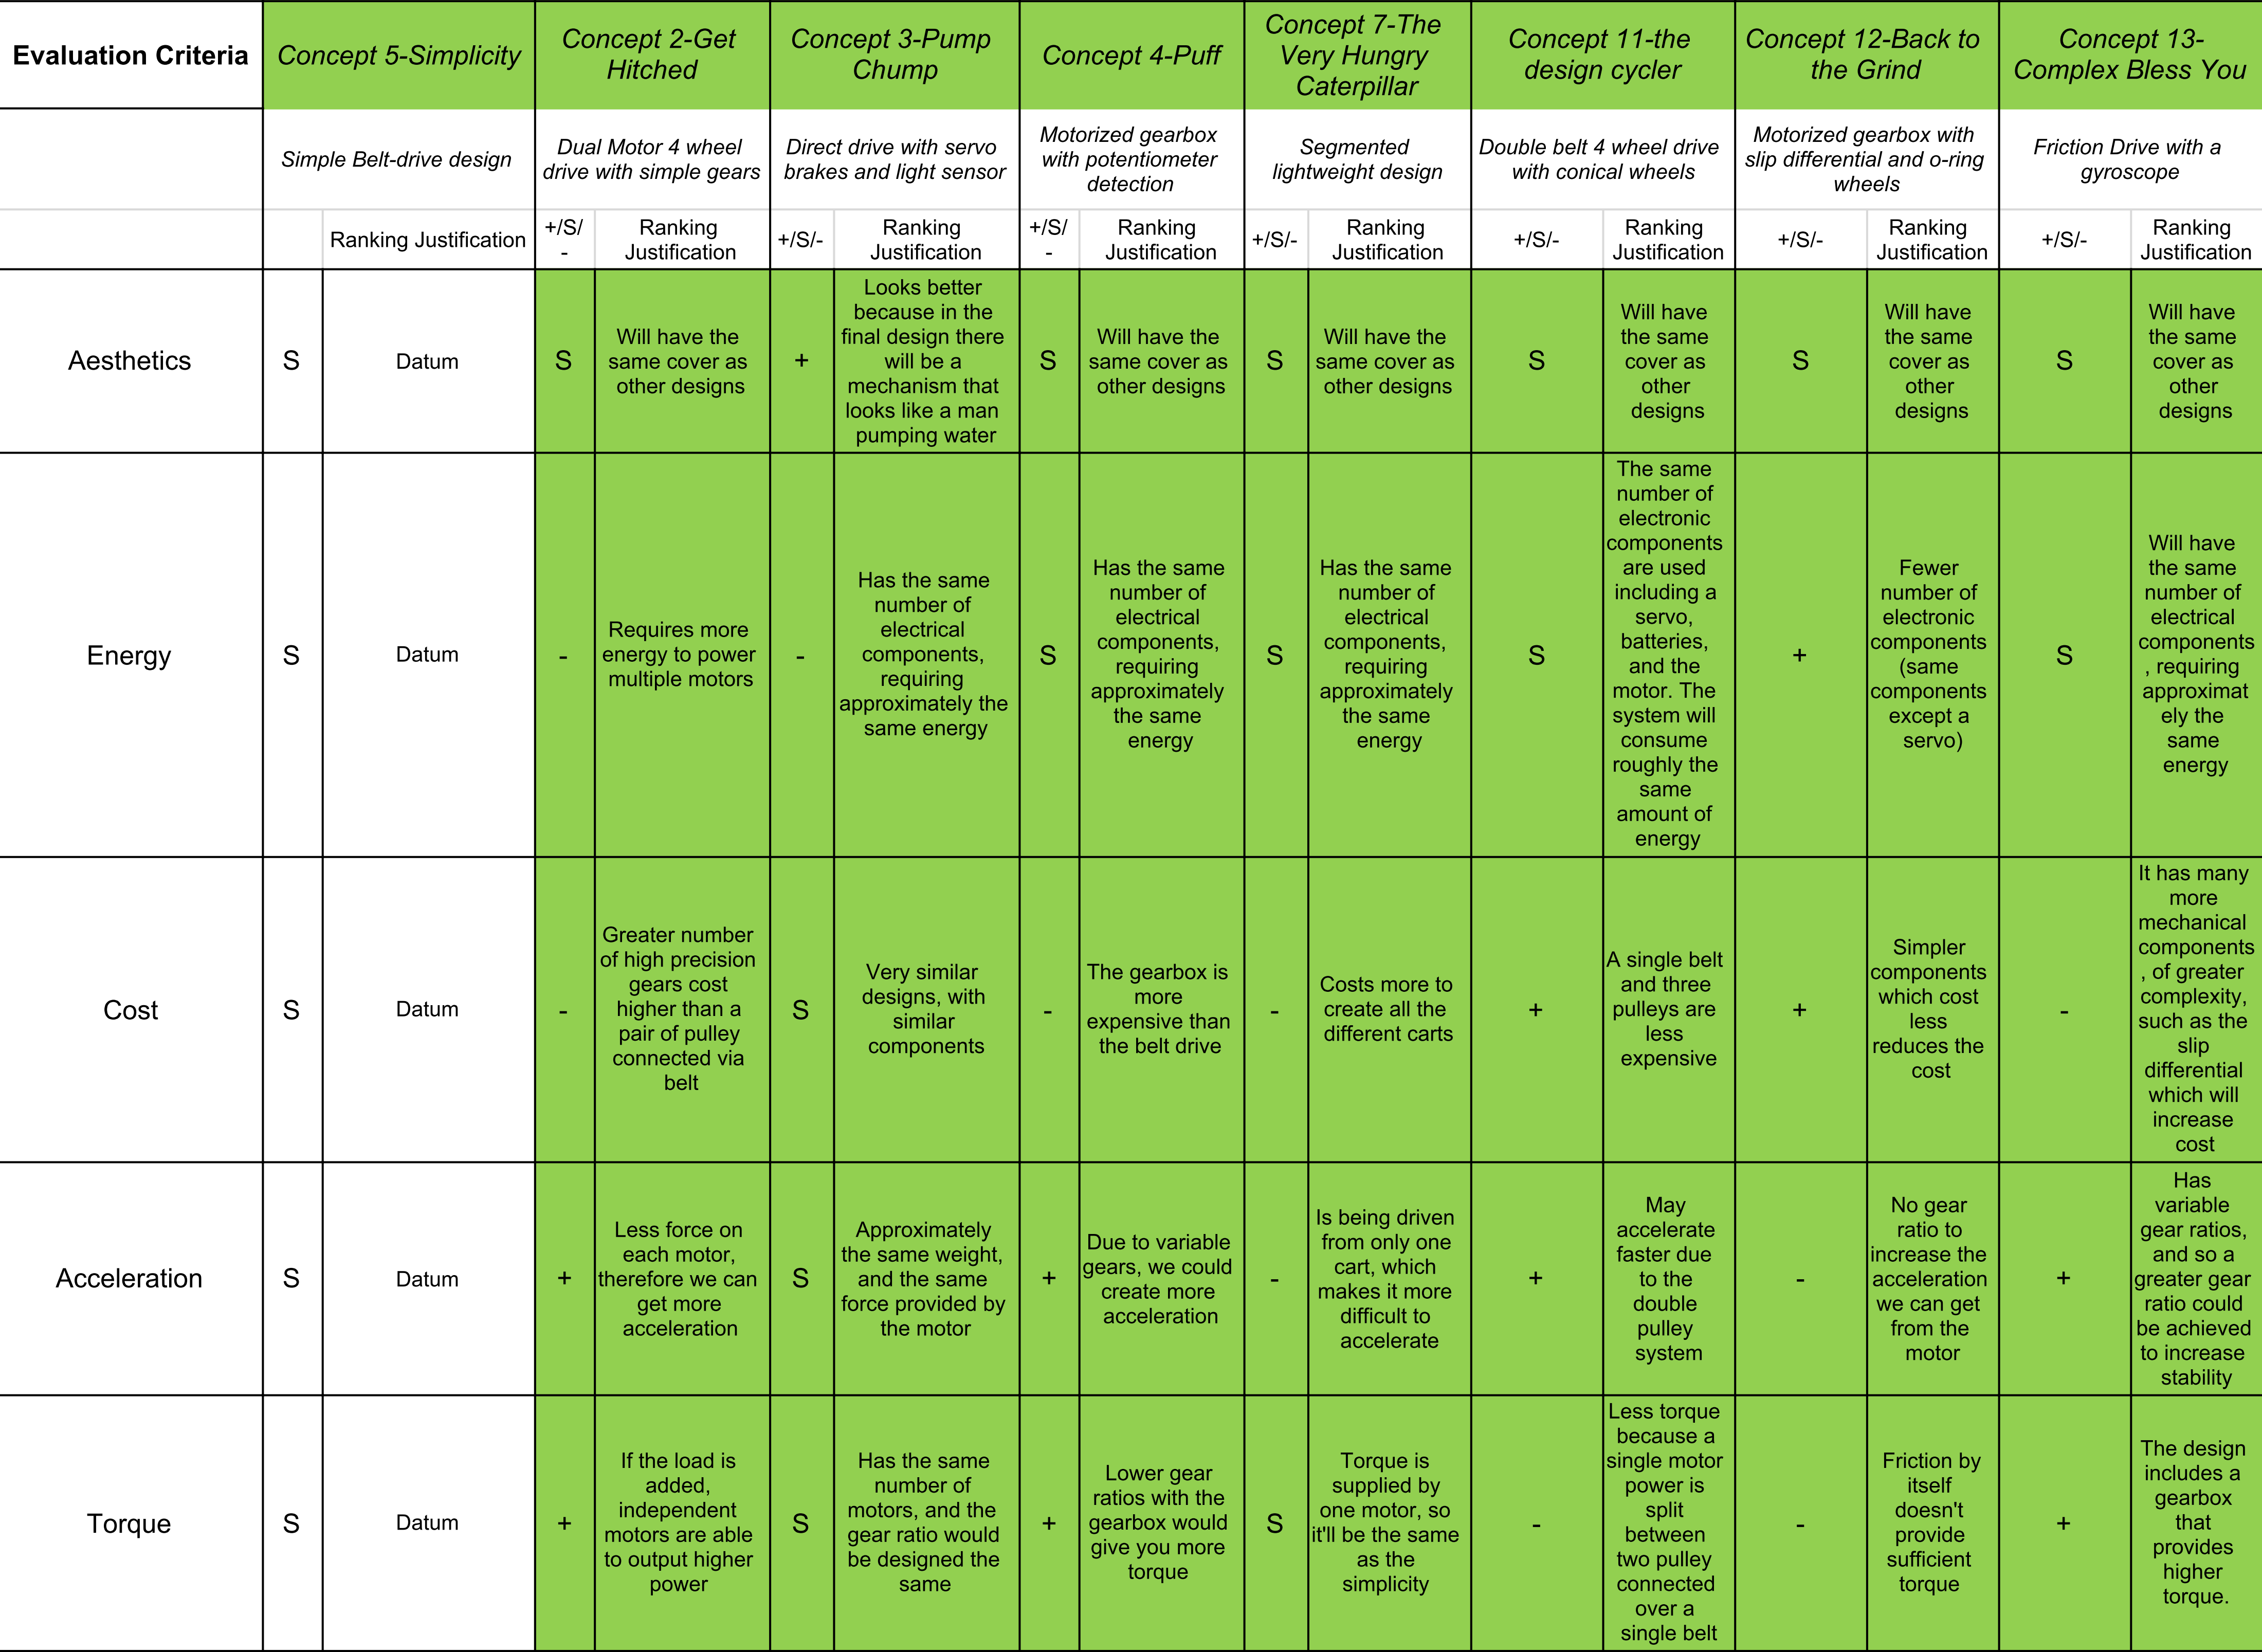
\includegraphics[width=\textwidth]{../../res/img/pugh1-1}
			\captionof{table}{Pugh Chart using Simplicity as a Datum}
			\label{app/table:pughsimplicity1}
		\end{minipage}
	\end{sideways}
\end{center}
\mbox{} \begin{center}
\begin{sideways}
	\begin{minipage}{1.25\textwidth}
		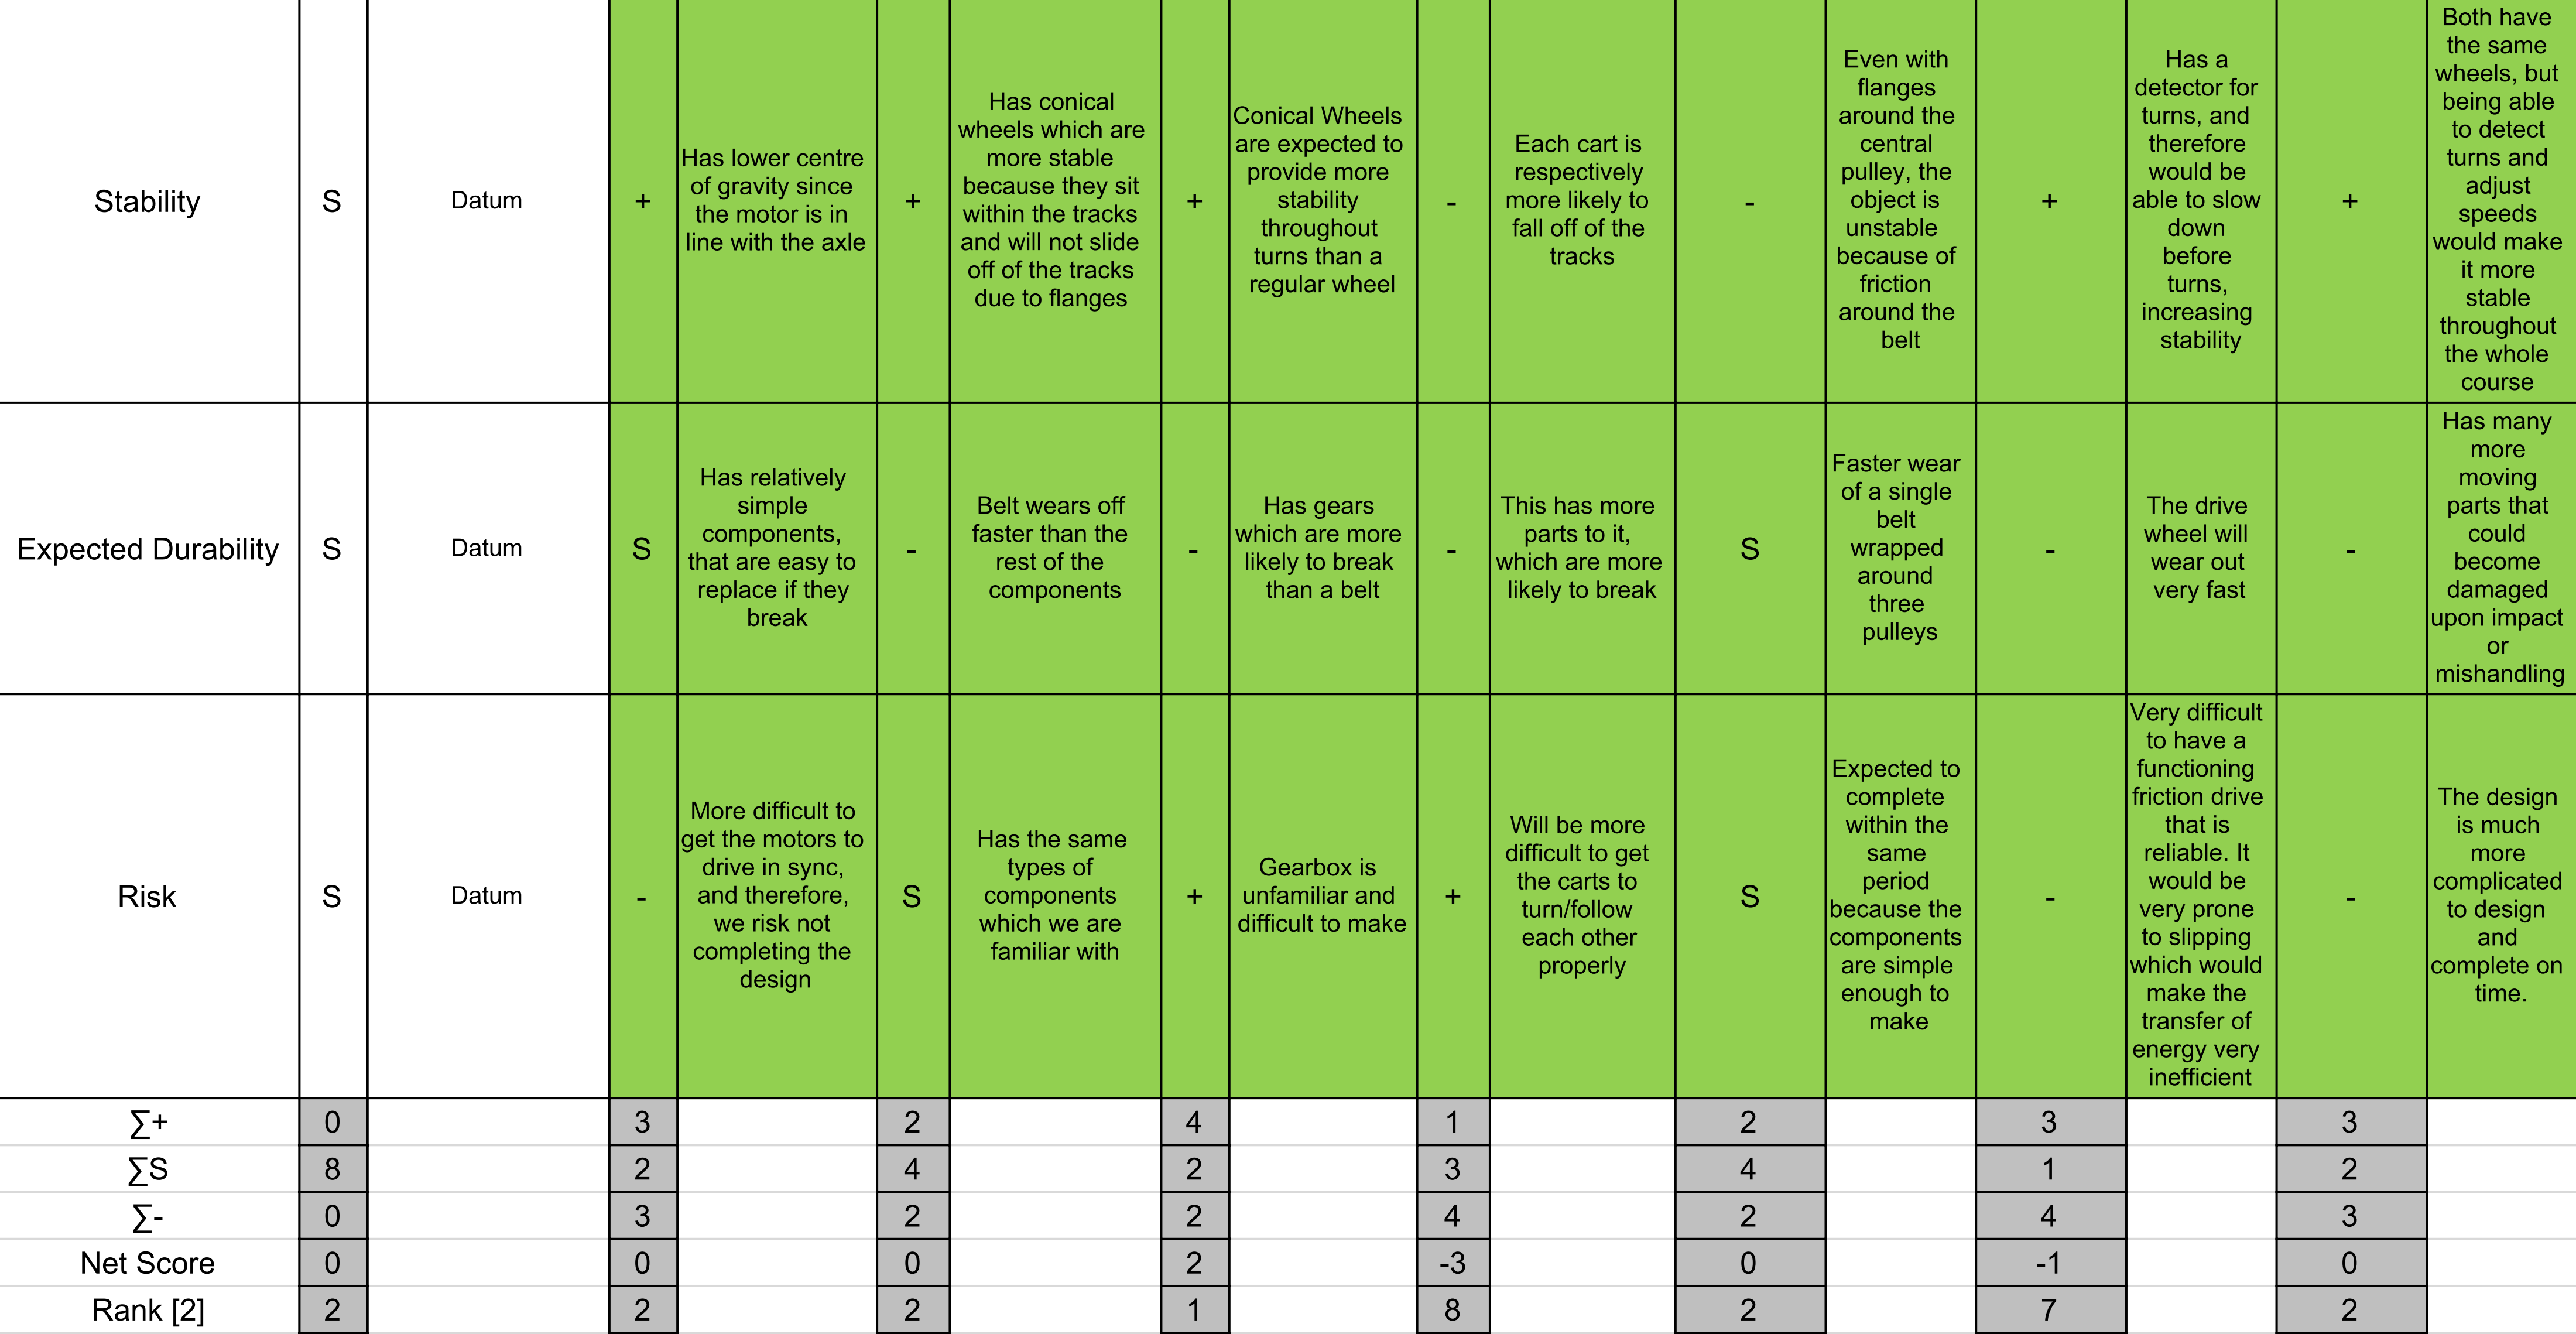
\includegraphics[width=\textwidth]{../../res/img/pugh1-2}
		\captionof{table}{Pugh Chart using Simplicity as a Datum}
		\label{app/table:pughsimplicity2}
	\end{minipage}
\end{sideways}
\end{center}
\mbox{} \begin{center}
	\begin{sideways}
		\begin{minipage}{1.25\textwidth}
			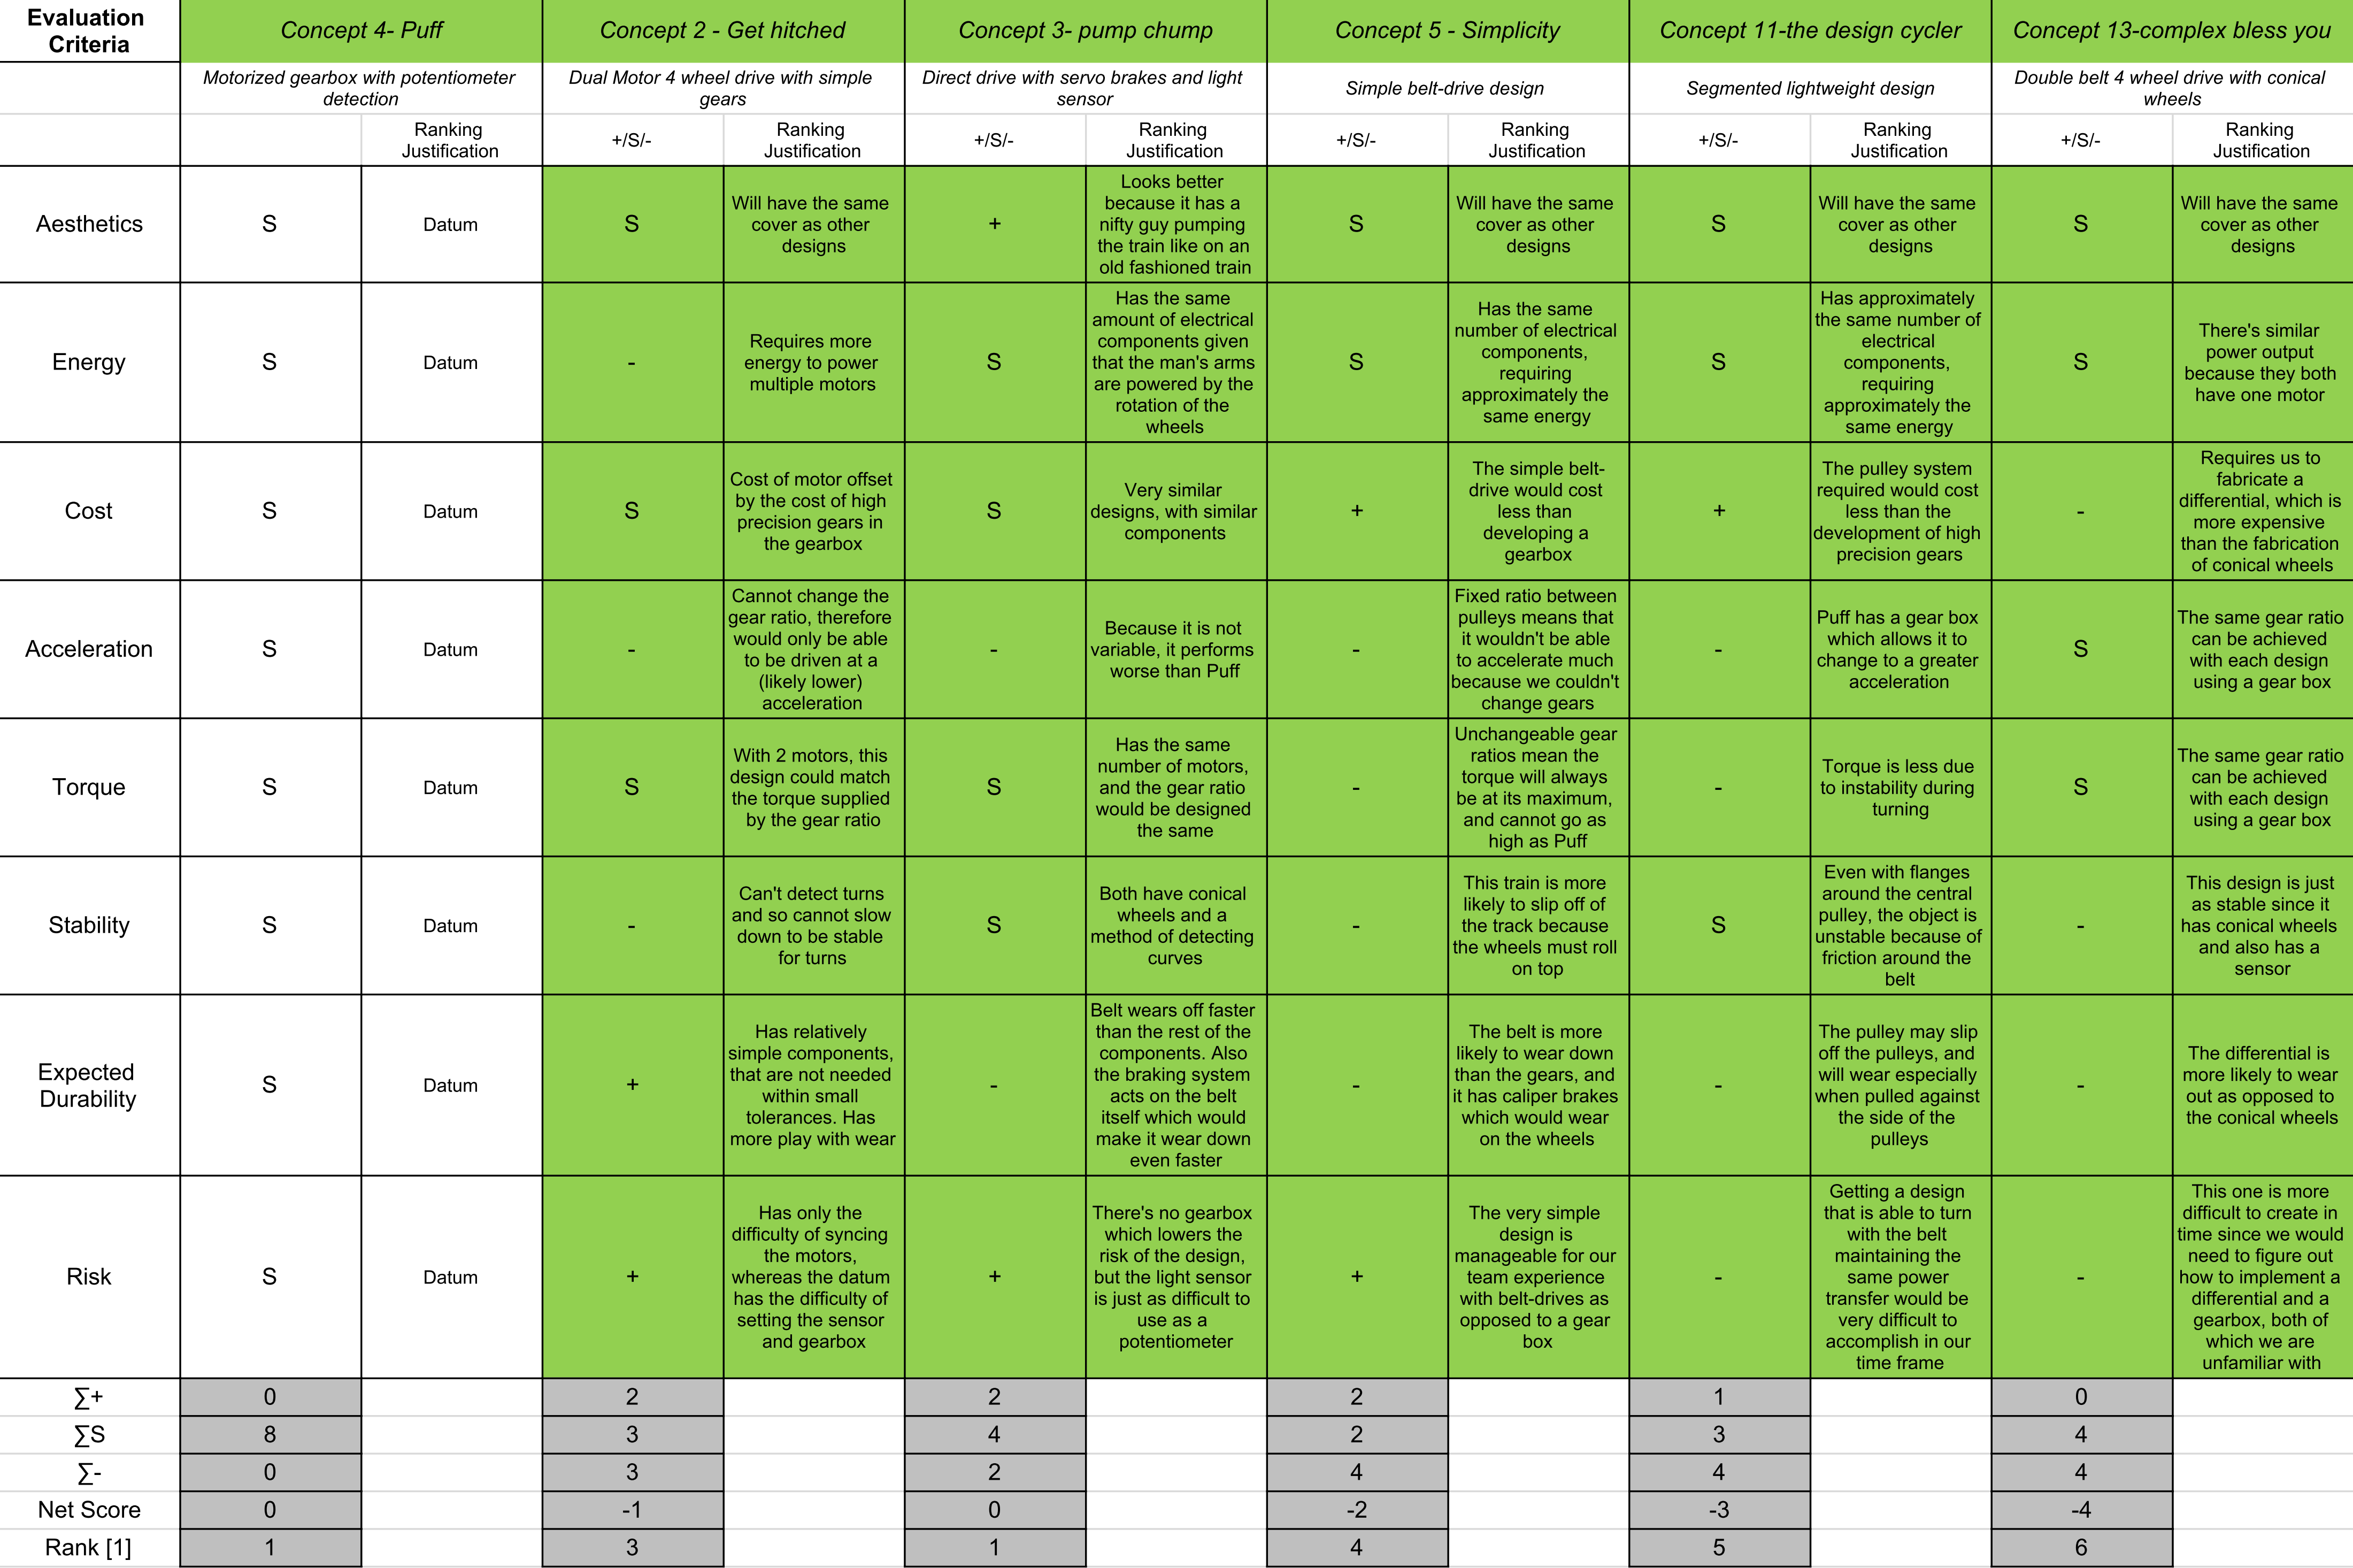
\includegraphics[width=\textwidth]{../../res/img/pugh2-1}
			\captionof{table}{Pugh Chart using Puff as a Datum}
			\label{app/table:pughpuff}
		\end{minipage}
	\end{sideways}
\end{center}


\end{document}
